\documentclass[conference]{IEEEtran}
\IEEEoverridecommandlockouts
% The preceding line is only needed to identify funding in the first footnote. If that is unneeded, please comment it out.
% \usepackage{cite}
\usepackage{amsmath,amssymb,amsfonts}
\usepackage{algorithmic}
\usepackage{graphicx}
\usepackage{textcomp}
\usepackage{xcolor}
\def\BibTeX{{\rm B\kern-.05em{\sc i\kern-.025em b}\kern-.08em
    T\kern-.1667em\lower.7ex\hbox{E}\kern-.125emX}}

\usepackage{tikz}
% \usetikzlibrary{shapes,arrows} % for the block diagram
\usetikzlibrary{shapes,arrows,fit,calc,positioning,automata}
\usetikzlibrary{backgrounds, calc,patterns,angles,quotes, babel} % f�r TSRL Bild
 %-------------------TIKZ KONFIGURATION----------------------------------
 \newcommand{\muxheight}{7em}
 \newcommand{\muxdist}{\muxheight/7}
 \newcommand{\blockwidth}{6em}
 \newcommand{\VarSysWidth}{2.1*\muxheight}
 \newcommand{\VarSysHeight}{1.2*\muxheight}
 \newcommand{\VarArrLen}{0.5cm}
 % for blocks with multiple inputs:
 \newcommand{\yarrowshift}{\blockwidth/8}

% \usepackage[
%       backend=biber,
%       style=numeric,
%       sortcites,
%       sorting=nty,
%       backref,
%       natbib,
%       hyperref
%   ]{biblatex}

% \addbibresource{BibTeX_database_BC-DS_nitr.bib}

\usepackage{float}
\usepackage[]{hyperref}
\hypersetup{
    colorlinks=false,
}

\usepackage{util}

\newcommand{\Aeff}{\ind{A}{eff} }
\newcommand{\vp}{\varphi}
\newcommand{\vpd}{\ind{\vp}{d}}
\newcommand{\Reff}{\ind{r}{eff}}
\newcommand{\abs}{|}


\begin{document}

\title{Iterative Learning Control \\ of a Pneumatically Driven Robot Joint%\\
% {\footnotesize \textsuperscript{*}Note: Sub-titles are not captured in Xplore and
% should not be used}
% \thanks{Identify applicable funding agency here. If none, delete this.}
}

\author{\IEEEauthorblockN{1\textsuperscript{st} Rainer Nitsche}
\IEEEauthorblockA{\textit{Robotics System Design} \\
\textit{Festo SE \& Co. KG}\\
Esslingen, Germany \\
rainer.nitsche@festo.com}
\and
\IEEEauthorblockN{2\textsuperscript{nd} Timo Heubach}
\IEEEauthorblockA{\textit{Robotics System Design} \\
\textit{Festo SE \& Co. KG}\\
Esslingen, Germany \\
timo.heubach@festo.com}
}

% <<FF>> **************************************************************
\maketitle
% *********************************************************************

\begin{abstract}
  The unique physical characteristics of pneumatic drives facilitate
  the creation of robots that are not only safe and lightweight but
  also intuitive to operate. However, pneumatic robots are due to the
  nonlinear behaviour hard to control. Especially friction plays a
  major role and limits the control performance of tracking a desired
  trajectory.  In this contribution the concept of {\em Iterative
    Learning Control (ILC)} is introduced and applied to a
  pneumatically driven joint build-in a pneumatic cobot. Iterative
  Learning Control is highly suitable to repeatable control tasks as
  they appear typically in robot applications \cite{Longman2000}. With
  this approach it is possible to almost perfectly track a given,
  repeatable trajectory.
\end{abstract}

\begin{IEEEkeywords}
  model-based control, robot control, flatness, iterative learning
  control, pneumatic robotics
\end{IEEEkeywords}

\section{Introduction}
Robot control tasks often follows a repeating trajectory. For this
kind of application the concept of learning from the error of the
previous control run lies at hand. That's why in the field of robot
control the concept of ILC is often used \cite{AhnChenEtAl2007}.

The concept of Iterative Learning Control is based on the idea that
repeated runs of a continuous task can be used to gradually improve
the performance of the control step by step.

The aim of ILC is to iteratively improve the control quality of such
systems through learning.

To achieve this, the error and the control signal of the previous
cycle are analyzed and used to adapt the new control signal. Due to
the fact that the new control signal is already calculated before each
cycle, it is possible to apply non-causal algorithms and filters.
This is a big adbantage compared to a classical feedback controller.
The ILC approach can be considered as a kind of feedforward control,
since the control signal only depends of the control error of the
previous cycle.

The ILC approach belongs to the class of feedforward controllers and
can be extended in the sense of a a two-degree-of-freedom structure by
adding a feedback component.  A classic PID controller can be used
here, for example. Through a combination of feedforward and feedback
control, the control control peformance and disturbance rejection can
be improved significantly. This is achieved, as the ILC controller
reduces the periodic errors and the feedback controller compensates
the disturbances \cite{ILCGlueck2015}.  For the feedback controller a
flatness-based approach in the sense of \cite{FliesLevineEtAl1995} is
used to have a model-based tracking controller of high performance. In
a second step an ILC approach is introduced to almost perfectly track
a desired repetitive trajectory.

This two-degree-of-freedom concept will be applied to a pneumatic
robot joint and tested in experiments. The achieved performance is
outstanding.



% *****************************************************************
\section{Control Task}
% *****************************************************************
For pneumatic robots so far, only fluidic muscles \cite{Tondu2005},
\cite{BouSaba2018} or bellows for soft robots \cite{Falkenhahn2017}
are employed.  However, pneumatic robots with rigid links and flexible
rotary joints, reducing model complexity and kinematic uncertainty,
are less common found in the literature.  This approach facilitates
the development of real-time feasible model-based controllers and has
the potential to achieve higher precision. First of all, the robot
must be able to track trajectories, which is usually a repetitive
task. For pneumatic manipulators with coupled joints, this control
taks is only reported to be ralizable with less accuracy
\cite{Bobrow1998} \cite{Mattiazzo2002} \cite{Taghia2012}.

Iterative learning control approaches for robots are highly suitable
\cite{Owens2016} but not yet reported for pneumatically driven robots,
but for other industrial applications, \eg. \cite{STADLER2022105071}.

% <<fig>> ************ Octopus Gripper *******************************
\begin{figure}[htbp]
  \centerline{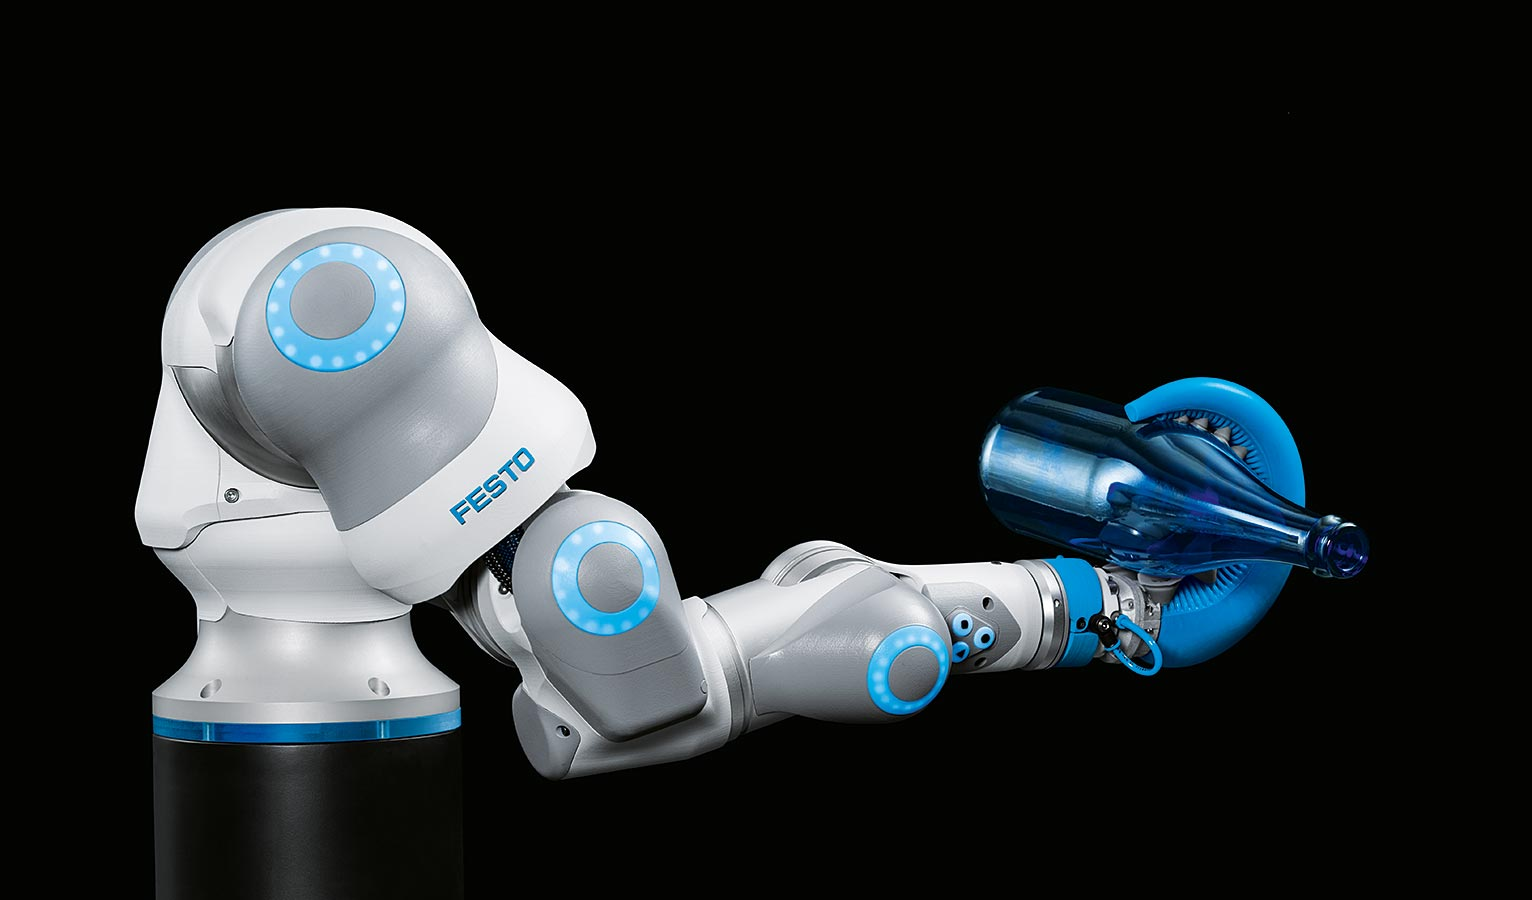
\includegraphics[width=\columnwidth]{./pictures/octopusgripper.jpg}}
\caption{Pneumatic Cobot from Festo (2020).}
\label{fig:Octopus}
\end{figure}
% ******************************************************************

% \newpage

% As a drafted version the paper of Steinboeck can be used \cite{STADLER2022105071}
% \begin{verbatim}
% https://www.sciencedirect.com/science/article/pii/S0967066122000041?via%3Dihub
% \end{verbatim}

\subsection{Model of the Pneumatic Robot Joint}

In this research a single joint (\cf. Fig.~\ref{fig:pJointScheme}) of
a pneumatic robot (\cf. Fig.~\ref{fig:Octopus}) is considered.  In
this pneumatically driven revolute joint, the two pressure chambers
are separated by a swivel wing of area $\Aeff$ and an effective radius
$\Reff$, which is semi-rotatable to $\pm 135^\circ$. The pressure
difference between the two chambers $1$ and $2$ of the joint generates
a driving torque
\begin{equation}\label{drvtrq}
  \tau(p_1, p_2) = \Aeff \; \Reff \; (p_1-p_2).
\end{equation}


The pressure in each chamber is set individually by a massflow
$\dot m_{1,2}$ into or out of the chamber with a pneumatic valve. A
more detailed overview of the pneumatic model can be found in
\cite{Hoffmann2021}.

The governing equations of the rotary joint model are:
\begin{subequations} \label{pJointMdl}
  \begin{align}
    % \dot q  & =  q} , \\
    \label{ddphi}
    \ddot \vp  & =  \frac{\Aeff\Reff (p_1-p_2) - \ind{\tau}{f}(\dot\varphi)}{J} , \\
    \label{dp1}
     \dot p_1 &= \frac{n ( R T \dot{m}_1 - p_1 \Aeff \Reff \dot\vp )}{ 
                \Aeff\Reff\;(\;\abs{\vp_{\mathrm {max}}}+\vp\abs)}  \\
    \label{dp2}
    \dot p_2 &= \frac{n ( R T \dot{m}_2 + p_2 \Aeff \Reff \dot\vp )}{ 
               \Aeff\Reff\;(\;\abs{\vp_{\mathrm {max}}}-\vp\abs)} ,
  \end{align}
\end{subequations}
where $\ind{\tau}{f}$ is the friction torque
(\cf. Figure~\ref{fig:pJointScheme}), $n$ is the polytropic exponent,
$R$ the specific gas constant, and $T$ the temperature. The valves are
installed next to the drive, so the tubes are short and the mass flow
to and from the pressure chamber are considered to be equal to the
mass flow set by the valves.
% \eqref{ddphi}\eqref{dp1}\eqref{dp2}
% See also \cite{HoffmannIFAC23}, and  \cite{Hoffmann2023}.
% <<FF>> *********************************************************
\begin{figure}[htbp]
  \setlength{\unitlength}{1cm}
   \begin{picture}(5,6)
  % \centerline{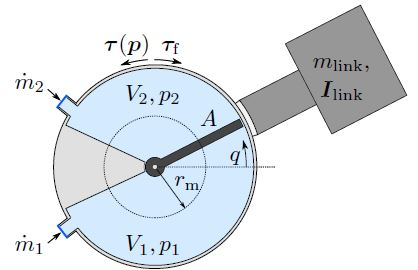
\includegraphics[width=\columnwidth]{./pictures/pJoint.jpg}}
     \centerline{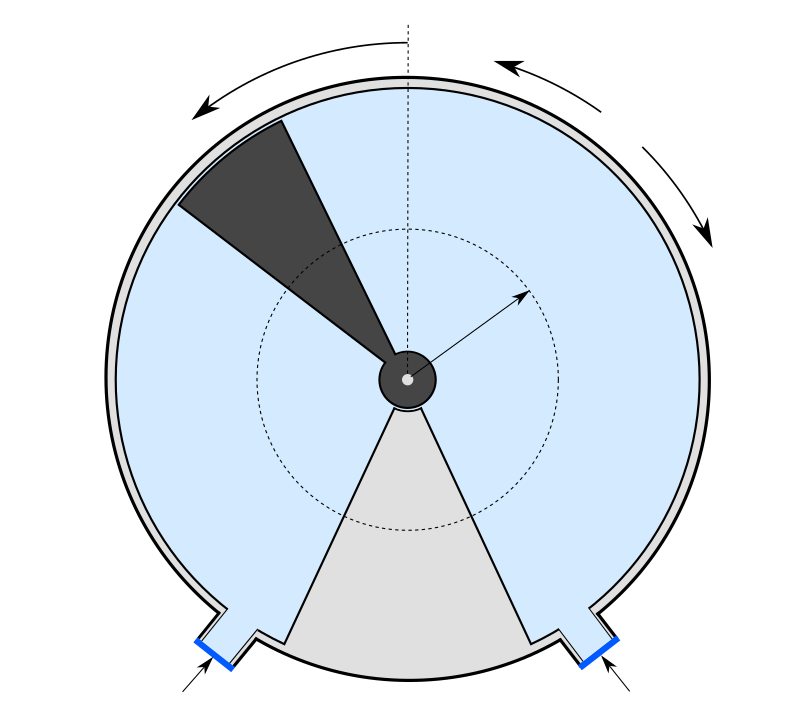
\includegraphics[scale=0.3]{./pictures/Struk_Zylinder2.png}}
 % Beschriftungen
   \put(-2.6,-.2){$\dot m_1$}
   \put(-6.2,-.2){$\dot m_2$}
   \put(-3.2,5.2){$\tau(p_1,p_2)$}
   \put(-2.1,4.2){$\ind{\tau}{f}(\vp)$}
   \put(-3.8,2.9){$\Reff$}
   \put(-5.2,4.5){$\Aeff$}
   \put(-5.2,5.5){$\dot \vp, \vp$}
   \put(-2.8,2.5){$p_1$}
   \put(-6.2,2.5){$p_2$}   
   \end{picture}
 \caption{Schematics of a pneumatic rotary joint.}
\label{fig:pJointScheme}
\end{figure}
% ******************************************************************

\begin{Remark}\label{rem:friction}
  In the following, the friction will be neglected for controller
  design, since the task of the ILC is to compensate the friction,
  which plays a crucial role in controlling the position of the
  pneumatic joint with high accuracy. \hfill $\square$
\end{Remark}


\section{Controller Design}

In a first step of the controller design a subordinary pressure
controller based on flatness is introduced. To control the position
$\varphi$ a simple linear $PI$ controller is added.

In a second step, a controller using the ILC approach is added to have
a better or almost perfect tracking behavior for repeating sequences
of the desired position $\vpd$.

The structure of the control loop can be seen in Fig.~\ref{fig:CtrlStrct}.

For the controller design of the position controller of the pneumatic
joint \eqref{pJointMdl}, the mass flows are the the control inputs
\begin{equation}\label{Uctrl}
  \uv = \left[\dot m_1, \dot m_2 \right]^T,
\end{equation}
and the state vector is defined as
\begin{equation}\label{states}
  \x = \left[\vp, \dot\vp, p_1, p_2\right]^T.
\end{equation}




\subsection{Flatness-based Approach -- Inner Loop}\label{FlatDesign}
According to \cite{Rothfus1997} a flatness-based controller for the
pressures in chamber 1 and 2, respectively, are designed. The
underlying flatness-based pressure controllers for the chambers can be
designed independently, since both chambers are only coupled via the
position $\vp$ and velocity $\dot \vp$ of the swivel. For the
controller design these states can be considered as variable
parameters as proposed in \cite{Falkenhahn2017}.

It is easy to see from \eqref{dp1} that $p_1$ is a flat output for chamber~1, \ie.:
\begin{subequations}\label{y1flat}
  \begin{align}
    y_1 & = p_1 \\
    \dot y_1 &= \dot p_1 = \frac{n}{V_1(\vp)} \left(R T \dot m_1 - p_1 \dot \vp \ind{V}{spec}\right) = \theta_1(p_1, \dot m_1,\vp, \dot\vp),
  \end{align}
\end{subequations}
with $V_1(\vp)= \Aeff\Reff\;(\;\abs{\vp_{\mathrm {max}}}+\vp\abs)$
and $\ind{V}{spec} = \Aeff\Reff$.

By introducing a new input $\nu_{p_1}$ for $\dot p_1$, one gets:
\begin{equation}\label{nu1}
 \dot p_1 =  \frac{n}{V_1(\vp)} \left(R T \dot m_1 - p_1 \dot \vp \ind{V}{spec}\right)  = \nu_{p_1}
\end{equation}
The nonlinearity of chamber~1 can now easily linearised by feedback
solving \eqref{nu1} for the system input:
\begin{equation}\label{eta1}
 \dot m_1 = \frac{V1(\vp)}{n R T}\left( \nu_{p_1} - \frac{n p_1 \dot V_1(\dot \vp)}{V_1(\vp)}   \right) = \eta_1(\vp,\dot \vp,p_1,\nu_{p_1}).
\end{equation}
The same holds for the second chamber, \ie.:
\begin{equation}\label{linFB}
  \dot m_i = \eta_i(\vp,\dot \vp,p_i,\nu_{p_i}), \quad i \in \{1,2\}.
\end{equation}
Applying \eqref{linFB} to the model of the rotational joint
\eqref{pJointMdl} the systems is in Brunovsky canonical form
\cite{Isidori1995}, \cf. Figure~\ref{fig:Bruno}.

For model of the rotational joint, linearized by feedback,
\ie. \eqref{pJointMdl} with \eqref{linFB}, a linear controller for the
pressures can easily designed:
\begin{equation}\label{linPresCtrl}
\nu_{p_i} = \dot p_{i,\mathrm{d}} - k_i (p_i - p_{i,\mathrm{d}}) , \quad i \in \{1,2\}.
\end{equation}

%<<fig>> ****************** Bruno *************************************
\begin{figure}[tbp] %[htbp]
  \begin{center}
  \unitlength1mm
  % \setlength{\fboxsep}{0pt}
  %\fbox{
   \begin{picture}(30,16)
 % Beschriftungen
     \put( 0, 7.5){\makebox(10, 5){${\nu}_{p_i}$}}
       \put( 20, 7.5){\makebox(10, 5){$p_i$}}     
      \multiput( 10, 0)(20, 0){1}{\framebox(10,15){$\D\int$}}
      \multiput(  0, 7.5)(20, 0){2}{\vector(1,0){10}}
   \end{picture}
%   }
 \end{center}
   \caption{Brunovsky normal form for the pneumatic joint, \ie. \eqref{pJointMdl} with  \eqref{linFB}.}
\label{fig:Bruno}
\end{figure}
% *****************************************************************

% *****************************************************************
\emph{Position Control for the Linearized System}\\[1pt]
% *****************************************************************
To control the postion of the rotational joint, a simple linear controller is used:
\begin{subequations}\label{taupi}
  \begin{align}
               e &= (\vpd-\vp), \\
  \ind{\tau}{PI} &= \ind{k}{p} e + \ind{k}{I}\int e \; \mathrm{d}t. 
 \end{align}
\end{subequations}



% **************************************************************
\subsection{Iterative Learning Control -- Outer Loop}
% **************************************************************

% <<fig>> *********************************************************
\begin{figure*}[tbp]
\centerline{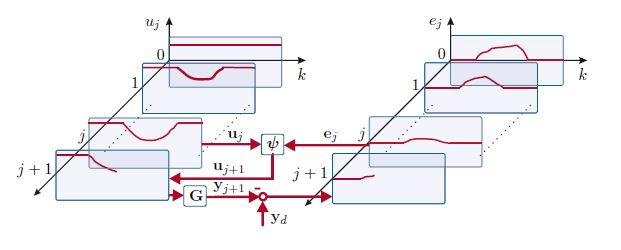
\includegraphics{./pictures/ILCillu.jpg}}
\caption{Illustration of the ILC concept \cite{ILCGlueck2015}.}
\label{fig:illuILC}
\end{figure*}
% ******************************************************************


In the controller desing so far, no friction model
(\cf. Remark~\ref{rem:friction}) or other model uncertainties has been
considered. To address this issues an Iterarive Lerning Control
approach is introduced and applied to control the position of the
pneumatic robot joint.

\begin{Remark}\label{rem:ILCrepeating}
  One condition to successfully apply an ILC concept to an application
  is, that the trajectories are continuously repeating. Another
  condition is, that the system to be controlled is stable. That is why
  an underlying controller, \eg. the flatness-based pressure and
  position controller is applied to stabilize the system. \hfill $\square$
\end{Remark}

\emph{Iterative Learning Control works as follows:} In each iteration
$\left(j=0,1,\ldots\right)$ a feedforward control value $\uv_{j+1}$ is
calculated.

% <<fig>> ******************* CtrlStruct Blockschaltbild *******************
% <<fig>> *********************************************************
\begin{figure*}[tbp]
  \unitlength1mm
  \begin{picture}(40,40)
    \centerline{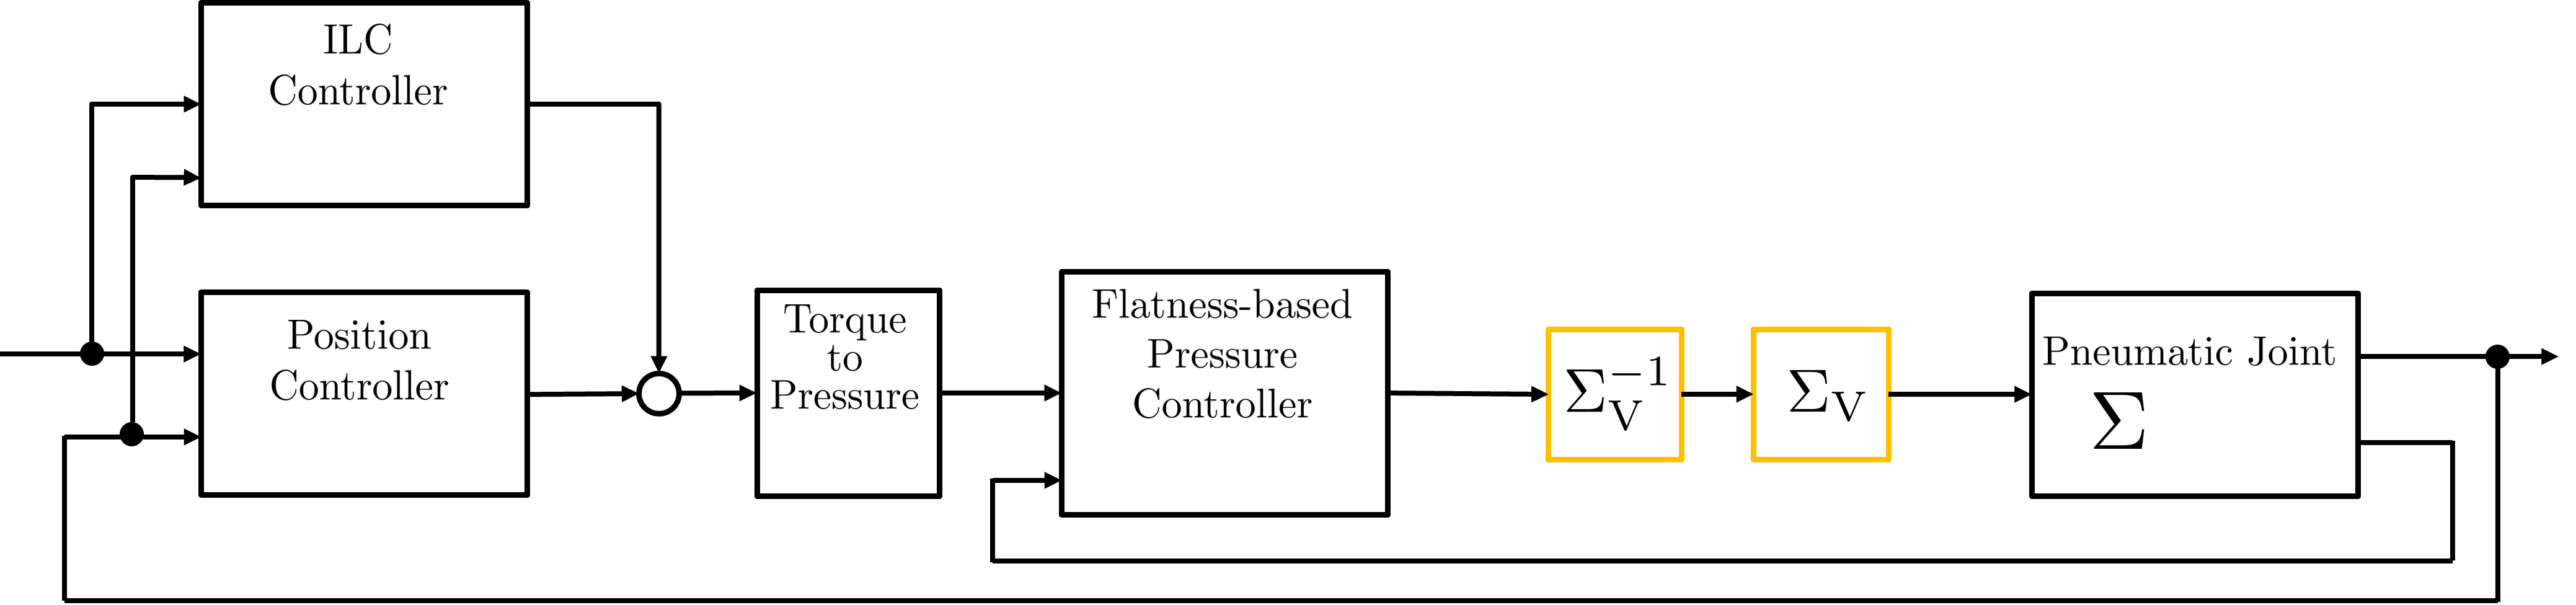
\includegraphics[scale=0.55]{./pictures/BlockSchaltFrame.png}}
    % Beschriftung von rechts nach links
    % Joint Modell *************************
    \put(-15,19){$\vp$} % Outputs
    \put(-65,4.5){$p_1,p_2$}  % KOmmt mehr in die Mitte    
    \put(-29,11.5){\eqref{pJointMdl}} % Innen
    \put(-47,16.2){$\dot m_1$} %  Inputs
    \put(-47,11){$\dot m_2$}
    % FlatnessBased Controller
    \put(-82,16.2){$\ind{\dot m}{1}$} %  Outputs
    \put(-82,11){$\ind{\dot m}{2}$}
    \put(-100,8.5){\eqref{linFB}, \eqref{linPresCtrl}} % Innen
    \put(-113,20){$\ind{p}{1,d}$} % Inputs
    \put(-113,16.5){$\ind{p}{2,d}$} % Inputs
    % Torque 2 Pressure
    \put(-124,9){\eqref{tau2pd}} 
    \put(-130.5,16){$\tau$}    % Input tau
    % Summation
    \put(-141,16){$\ind{\tau}{PI}$}    % Input tauPI
    \put(-141,36){$\ind{\tau}{ILC}$}    % Input tauILC
    % PI Pos Ctrl
    \put(-157,9.5){\eqref{taupi}}   % Eqn
    \put(-178,8){$\vp$}   % phi
    \put(-178,19){$\vpd$}   % phi
    % ILC Controller
    \put(-157,30){\eqref{eq:ilc_diskret}} % Innen    
  \end{picture}
  \caption{Overall control structure. The compensation of the valve behavior,
    \ie. $\ind{\Sigma}{V} \circ \ind{\Sigma}{V}^{-1}$, is not
    considered here.}
\label{fig:CtrlStrct}
\end{figure*}
% ******************************************************************

%%% Local Variables:
%%% mode: latex
%%% TeX-master: "../robotJointILC"
%%% End:     % \label{fig:CtrlStrct}
% **************************************************************************

To do this, the error $\e_j$ and the control $\uv_j$ must be
determined and stored.  The output error
\begin{equation}
	\label{eq:e_yd_ym}
	\e = \y_\mathrm{d} - \y_\mathrm{m} \equiv
             \boldsymbol{\varphi}_\mathrm{d} - \boldsymbol{\varphi}
\end{equation}
is calculated from the difference between the desired signal
$\y_\mathrm{d}$ and the measured signal $\y_\mathrm{m}$.  In
Fig.~\ref{fig:illuILC} the sequences of the ILC approach is
illustrated \cite{ILCGlueck2015}.

In each iteration, the control $\uv_{j+1}$ is calculated by the
function $\bpsi\bigl(\uv_j,\e_j(\uv_j)\bigr)$. The new control
therefore only depends on the previous iteration.

The resulting control signal is applied to the system $\G$ in order to
measure the output $\y_{\mathrm{m},j+1}$. Using the setpoint signal
$\y_\mathrm{d}$, the new output error $\e_{j+1}$ is determined and
stored temporarily. At the same time, the control signal $\uv_{j+1}$
is also saved.

This process can be repeated as often as required, since the goal of
this procedure is to adjust the feedforward control $\uv$ such that
the output error $\e$ converges to zero.

For the computation of the control signal $\uv$ a minimization task is
used (\cf. \cite{ILCGlueck2015}). To do this, a gain matrix
$\Lm \in R^{N \times N}$ and a filter matrix $\Q \in R^{N \times N}$
is defined, where $N$ is the number of samplings during one iteration.

The ILC law depends on the relative degree $r$ of the system.  For
linear systems, the relative degree can be calculated by
\begin{equation}\label{eq:r}
  r = n-m,
\end{equation}
where the highest exponent of the numerator polynomial of the transfer
function is given by $m$ and the highest exponent of the denominator
polynomial is given by $n$.

For discrete-time systems, $r=1$ always applies.  It can therefore
also be interpreted as a delay.

In practical applications, in addition to the delay due to the
relative degree $r$ of the system, delays can also occur due to
digital-to-analog or analog-to-digital conversions. This delay is
given by the number of sampling steps $w$ required for the conversion.
This means that a total delay
\begin{equation}  \label{eq:m}
  v = r + w
\end{equation} can be introduced and taken into account in the ILC law.

By introducing

\begin{align}
	\label{eq:u_vec}
	\uv_j &= \bigl[u_j[0] \quad u_j[1] \,  \ldots \, u_j[N-1] \bigr]^T \in R^{N \times 1} \\
	\y_{\mathrm{d},j} &= \bigl[y_{\mathrm{d},j}[v] \quad y_{\mathrm{d},j}[v+1] \, \ldots \, y_{\mathrm{d},j}[v+N-1] \bigr]^T \in R^{N \times 1} \\
	\y_{\mathrm{m},j} &= \bigl[y_{\mathrm{m},j}[v] \quad y_{\mathrm{m},j}[v+1] \, \ldots \, y_{\mathrm{m},j}[v+N-1] \bigr]^T \in R^{N \times 1} \\
  \e_{j} &= \y_{\mathrm{d},j} - \y_{\mathrm{m},j} \nonumber \\
        & = \bigl[e_{j}[v] \quad e_{j}[v+1] \, \ldots \, e_{j}[v+N-1] \bigr]^T \in R^{N \times 1}, \label{eq:evec_def}
\end{align}
the ILC control law is given in lifted representation:
\begin{equation}
	\label{eq:ilc_lift}
	\uv_{j+1} = \Q\left(\uv_j + \Lm \e_j\right).
\end{equation}


The gain matrix $\Lm$ has the task of calculating the influence of the
output error $\e_j$ in relation to the previous control $\uv_j$. The
choice of matrix elements determine the influence of the output error
on the new feedforward-control.  The filter matrix $\Q$, on the other
hand, is used to suppress measurement noise and  repetitive
interference. It acts like a low-pass filter that only allows low
frequencies to pass through and filters out high frequencies. \\

The ILC law \eqref{eq:ilc_lift} can also be specified in the discrete
form:

\begin{subequations}
  \label{eq:ilc_diskret}
  \begin{align}
    u_{j+1}[k] & = q[k] \bigl(u_j[k] + l[k] \, e_j[k+v]\bigr),\\
    \ind{\tau}{ILC} & =  u_{j+1}[k] \label{tauILC}
    \end{align}
\end{subequations}

where $k = 0,1,\ldots,N-1$ is the sampling index.


% *****************************************************************
\subsection{Splitting the torque into chamber pressures}
% *****************************************************************
The output of the controllers \eqref{taupi} and \eqref{tauILC}
are torques which has  to be added and then converted / split into some
feasible pressure demands for the underlying pressure controller
\eqref{linPresCtrl}, \ie.:
\begin{equation}\label{tauOverall}
\tau = \ind{\tau}{PI} + \ind{\tau}{ILC},
\end{equation}

\begin{subequations}\label{tau2pd}
  \begin{align}
               \ind{p}{1,d} &= \ind{p}{m} + \frac{\tau}{2\;\ind{V}{spec}},\\
               \ind{p}{2,d} &= \ind{p}{m} - \frac{\tau}{2\;\ind{V}{spec}},
 \end{align}
\end{subequations}
while $\ind{p}{m}$ is the so-called mean pressure, which has to be
defined appropriately.
\begin{Remark}\label{rem:pm}
  The pressures $p_i$ range around this mean pressure. Note, this mean
  pressure can be changed during time, depending on the state of the
  robot or joint, \ie. $\ind{p}{m} = \ind{p}{m}(\x,t)$. In this case,
  this is a nonlinear MIMO controller. \hfill$\square$
\end{Remark}

\vspace*{2mm}

The overall control structure can be seen in
Fig.\ref{fig:CtrlStrct}. The compensation of the nonlinear valve
behavior, \ie. $\ind{\Sigma}{V} \circ \ind{\Sigma}{V}^{-1}$, is not
considered here. A detailled description of those mass flow
controllers acting on the valve $\ind{\Sigma}{V}$ can be found in
\cite{Hoffmann2021}.


% <<FF>> ***********************************************************
\section{Experimental Setup and Results}
% *****************************************************************
The introduced control concept was tested on an experimental setup as
seen in Fig.~\ref{fig:ExpSetUp}. This test bench consists of a single
pneumatic joint which is controlled within a rapid control prototyping
system from dSpace. The testbench consists of pressure control valve
for the supply pressure (1), buffer volume (2), flow sensors (3),
pressure sensor for the supply pressure (4), pneumatic valve with
valve controller (5), pressure sensor for the chambers (6,7),
pneumatic joint (8), and an interface PCB to the dSpace system.
% <<fig>> *********************************************************
\begin{figure}[bp]
  \centerline{\includegraphics[width=\columnwidth]{./pictures/Aufbau_pJoint.png}}
  \caption{Experimental Setup: the pneumatic joint (8) is controlled
    via a propotional Piezo valve (5) and a rapid-control-prototyping
    system from dSpace.}
\label{fig:ExpSetUp}
\end{figure}
% ******************************************************************

\subsection{Experimental Results}
% <<fig>> *********************************************************
% Script: C:\Users\nitr\OneDrive - Festo\home\papers\_ILC\pictures\plot_Messungen_dSpace.m
% Data:   ILC_Sollsignal_DR70_Shruti_fric.mat
\begin{figure*}[htbp]
\centerline{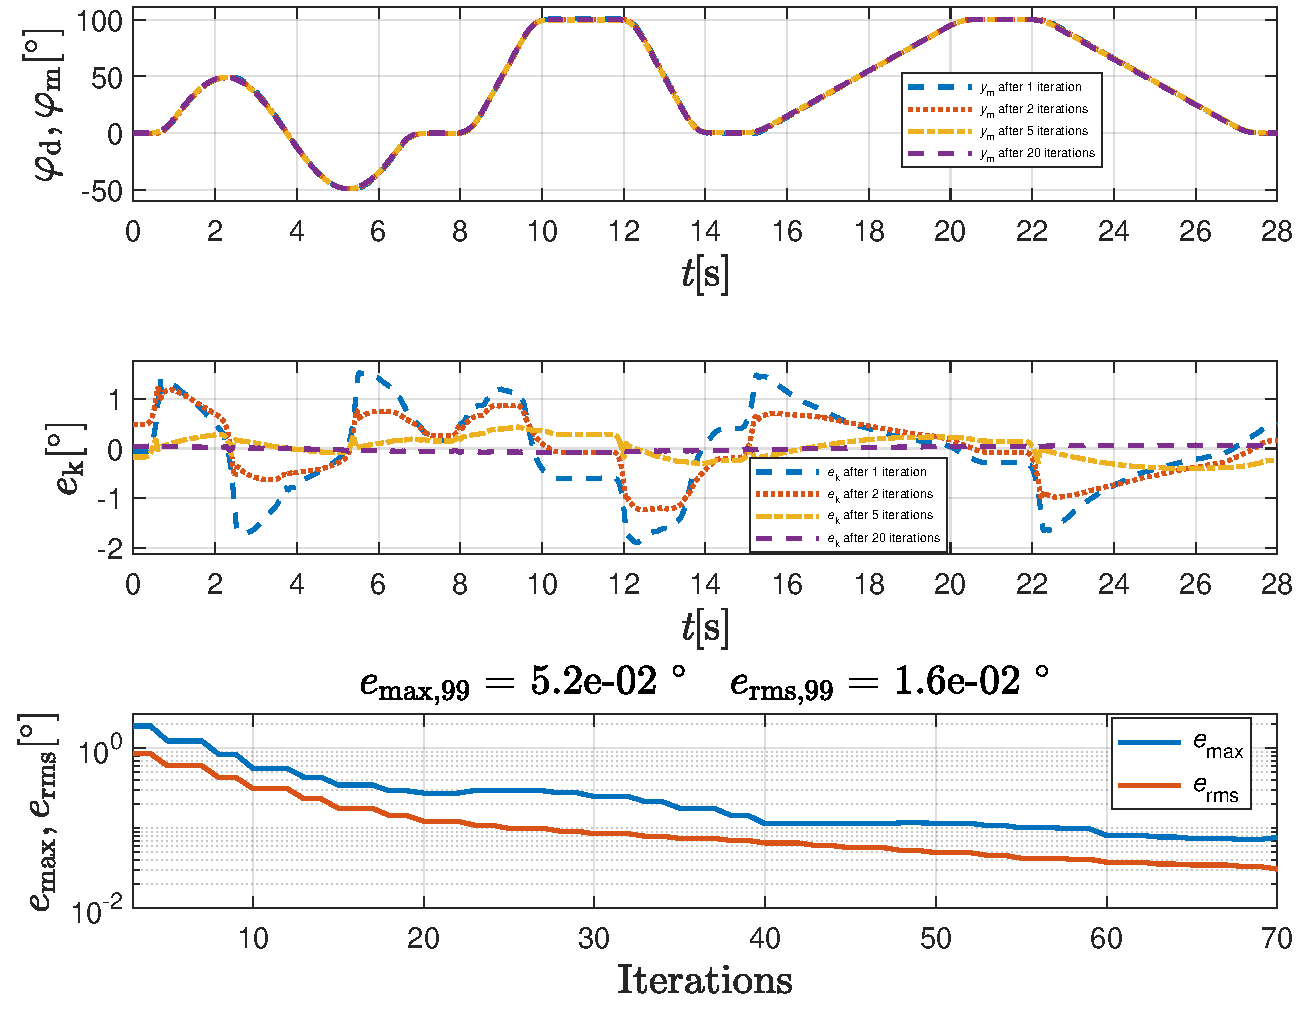
\includegraphics[scale=.7]{./pictures/dSpace_Messung_ILC_DR70_Shruti2.pdf}}
\unitlength1mm
\begin{picture}(0,0)
  \put(10,105){a)}
  \put(10,60){b)}
  \put(10,20){c)}
\end{picture}
\caption{Measurement resutls for a robot joint.}
\label{fig:ILC70Shruti}
\end{figure*}
% ******************************************************************

To test the proposed concept a typical test-trajectory is applied to
one of the swivel drives (Fig.~\ref{fig:pJointScheme}) of the
pneumatic robot (Fig.~\ref{fig:Octopus}). The test trajectory consists
of dynamic and stationary parts as can be seen in
Fig.~\ref{fig:ILC70Shruti}a. The trajectory tracking performance after
several interations (repetitions) can be seen in
Fig.~\ref{fig:ILC70Shruti}a and the tracking error in
Fig.~\ref{fig:ILC70Shruti}b. The performance after the first iteration
corresponds to the tracking performance of the flatness-based approach
only. A maximal tracking error of $\approx 1.5^{\circ}$ can be seen
after the first run, \ie. for the controller without the ILC
contribution. As can be seen clearly after several runs, the tracking
error decreases significantly. It can be seen clearly in
Fig.~\ref{fig:ILC70Shruti}b, that after 20 runs the tracking error is
almost zero. As mentioned in Remark~\ref{rem:friction}, no friction
compensation is implemented explicitly in the proposed control
concept, but the friction effects are compensated perfectly by the ILC
approach.



The evolution of the maximal control error and the
root-mean-square-error (rms) over several runs is almost neglectable,
as can be easily seen in Fig.~\ref{fig:ILC70Shruti}c. Note, the
ordinate in Fig.~\ref{fig:ILC70Shruti}c is scaled logarithmically.

\begin{Remark}\label{rem:ILCsmallDrive}
  Controlling the smallest drive in the robot, \ie. the drive for the
  hand-axis, is really a challenging task. For this rather tiny
  pneumatic actuator, the relation between the driving torque created
  by the pneumatics and the friction torque is extremely unfavorable.
  With the proposed ILC concept it was possible to achieve almost
  perfect tracking performance, even for the pneumatic drive of the
  hand-axis. \hfill $\square$
\end{Remark}




% <<FF>> ***********************************************************
\section{Summary}
% *****************************************************************

This paper successfully demonstrated that the use of Iterative
Learning Control Learning Control (ILC) improves the control
performance of repetitive motion significantly over time, even for
complex nonlinear systems.  By learning from previous cycles, the
control signal can be adapted for the next cycle, resulting in
improved control quality. Especially for pneumatic joints build in a
colaborative robot this concept is highly suitable, since friction and
model unaccuracies can be compensated almost perfectly.

A major advantage of the ILC algorithm is that it can be used in
parallel with any existing controller. One prerequisite for this is
that the desired trajectory must be identical for each cycle, which is
why the ILC approach is mostly used in a controller cascade in
parallel with the superimposed controller.

The acausal filtering in the ILC algorithm enables the control signal
to be filtered without phase shift. This is particularly important
when there is measurement noise in the controlled variable and when
used simultaneously with an existing controller.

It is successfully demonstrated, that a two-degree-of-freedom approach
(flatness-based pressure controller and ILC position controller) leads
to an almost perfect tracking performane for repetitive trajectories
for pneumatic robot joints.


% <<FF>> ***********************************************************
% \section*{References}
% *****************************************************************

% \newpage

\IEEEtriggeratref{12}

\bibliographystyle{plain}        % {alpha} Include this if you use bibtex 
\bibliography{BibTeX_database_BC-DS_4Codit}




\end{document}
